\section{Binarization}

A perfect binarized version of a papyrus image is defined by a background color and ink color, where the ink is black, and the background is white. Each pixel in an image is altered so that it is either black or white, depending on if it is ink or anything else (background). As no ground truth for ink was given to train on, all the methods for binarization are based on either pre-trained CNNs or algorithmic solutions utilized in similar problems.

\subsection{Clustering}

Clustering based binarization is performed with k-means clustering. For each image, the pixels of the image were placed in a 3d space with their red, green, and blue values being used to determine their location \seefig{pixelClustering}. Pixels were then clustered in groups using k-means clustering. The pixel cluster which contained the value closest to black was then utilized as the ink cluster, with all pixels not in that cluster being labeled as the background \seefig{binarizationClustering}.

\begin{figure}
    \caption{RGB Pixel Clustering In 3D Space}
    \label{fig:pixelClustering}
    \begin{center}
      \begin{subfigure}[b]{0.45\textwidth}
           \centering
           \caption{Pixel Clustering on An Image With Low Color Variation}
           \label{fig:goodPixelClustering}
           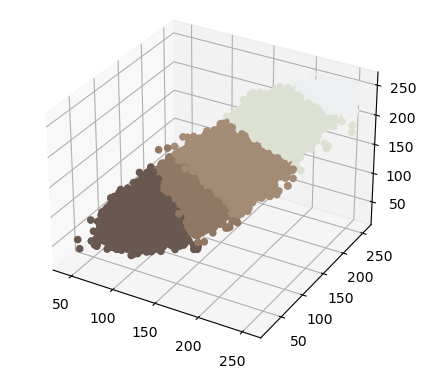
\includegraphics[width=\textwidth]{{binarization/good_pixel_clustering.png}}
       \end{subfigure}
       \hfill
       \begin{subfigure}[b]{0.45\textwidth}
           \centering
           \caption{Pixel Clustering on An Image With High Color Variation}
           \label{fig:badPixelClustering}
           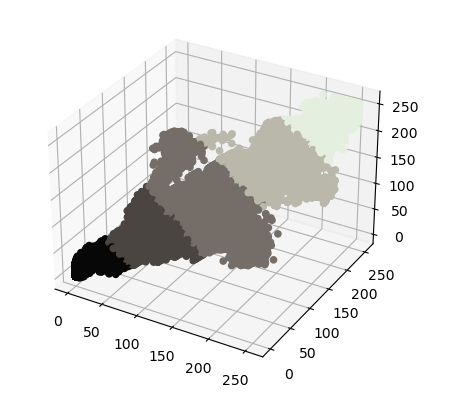
\includegraphics[width=\textwidth]{{binarization/bad_pixel_clustering.png}}
       \end{subfigure}
    \end{center}
    Two examples of clustering pixels using RGB color representation to place each pixel in space. These clusterings were generated using Gaussian Mixture Models (GMMs) clustering with $k=5$, with each cluster being colored by the color represented by location in RGB space of the cluster's centroid.
\end{figure}

\subsection{Gabor Filter}

Filtering based binarizations are generated utilizing the Gabor filtering  \cite{Gabor1949, Gabor1948} to find clusters of pixels that are not like those around them, which could be glyphs. Gabor filtering is based on a linear filter, but when multiple linear filters are grouped together with a set rotation applied to each subsequent filter, a 2d filter can be generated to generate a simplification of Gabor wavelets \cite{Gabor1949, Gabor1948}. Using these 2d filters, this method of binarization seeks to find features in an image that has a specific frequency, which in the case of glyphs might be the width or height of a single line in a glyph.

This method requires an assumption on the wave frequency that may generate the glyphs, so a manual heuristic method was utilized to generate the function that most accurately generated the correct wave for the images in the training dataset.

To utilize the approximation on a Gabor wavelet on the input, the input is read in and converted to a greyscale image before having the collection of Gabor filters applied. This reduces the channels from three to one and allows the Gabor wavelet approximation to work on the image. The outputs of each filter in the wavelet approximation are then averaged together to generate a new greyscale image, which can then be binarized using naive thresholding.

\subsection{Input Invarient Thresholding}

In a similar fashion to utilizing the Gabor filter or Gabor wavelet, thresholding utilizing an input invariant method, such as the one proposed by \cite{Bar-Yosef2005, Bar-Yosef2007} requires consistency in the input or a strong method for determining the correct threshold. Using clustering, as discussed above, could be a potential method to find a threshold, however the method them becomes a variant of clustering, so this method was not implemented past the initial stage of picking an arbitrarily chosen threshold value and binarizing the input by converting it greyscale and then binarizing the greyscale image by converting all values darker than the threshold to black and all other values to white.

\subsection{DP-Linknet}

Although it was out of the scope of this project to train a CNN to binarize an image, Convolutional Neural Networks have already been generated and trained on the problem of binarization of historical texts. DP-Linknet \cite{Xiong} is one such CNN, trained on historical texts and implemented in Python utilizing common deep learning tools such as PyTorch \cite{PyTorch} and Scikit-Learn \cite{Scikit}. As the Python source code for DP-Linknet is publicly available on \href{https://github.com/beargolden/DP-LinkNet}{GitHub}, it was a simple task to implement it into the project and add a simple API that integrates the CNN into the pipeline.

\textit{Note: All code contained in the} \code{src/binarization/dp\_linknet} \textit{folder is either directly from the GitHub reposity or highly based on that code. I take no credit for this code, as little of my own work was done to integrate the work of Xiong et al. into this project.}

% \subsection{BiNet}
% \todo{TODO}

\section{Glyph Bounding}

\subsection{Bounding Boxes}

Bounding boxes are represented internally by an object that holds the PASCAL Visual Object Classes (VOC) representation of a bounding box \seefig{pascalbbox}. Using this method of representation, compared to a tuple or list, allows for operations on bounding boxes to be standardized and for bounding boxes to be represented in a way that is abstracted from their format. Allowing this abstract bounding box format assists with the problem of having multiple constraints on how bounding boxes are utilized in the pipeline, such as importing and exporting COCO formatted bounding boxes \seefig{cocobbox}, calculating metrics based on PASCAL VOC formatted bounding boxes \seefig{pascalbbox}, and utilizing tools and methods that require YOLO formatted bounding boxes \seefig{yolobbox}. Bounding box objects are then able to utilize internal methods for operations such as finding the IOU (intersection over union) \seefig{IOU} between two bounding boxes, one dimensional IOU \seefig{1dIOU}, and generating cropped images from lists of bounding boxes.

\begin{figure}
    \caption{PASCAL VOC Bounding Box Examples}
    \label{fig:pascalbbox}
    \begin{center}
    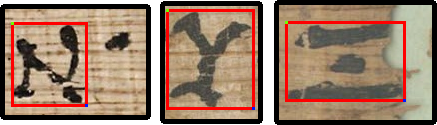
\includegraphics[width=0.75\textwidth]{{bounding/bbox_examples_pascal.png}}
    \end{center}
    Three examples of bounding boxes, on a $N$, $\Upsilon$, and a $\Xi$ (left to right). For these examples, the red lines denote the pixels that are inside of the bounding boxes. In the PASCAL VOC bounding box format, bounding boxes are described using the top left corner (marked in green) of the box in absolute pixels, and the bottom right corner of the box (marked in blue) in absolute pixels. In this example, the boxes shown above would be denoted in the PASCAL VOC format as follows: $N:(6, 13, 82, 97)$, $\Upsilon:(1, 3, 89, 103)$, $\Xi:(6, 16, 126, 96)$.
\end{figure}

\begin{figure}
    \caption{COCO Format Bounding Box Examples}
    \label{fig:cocobbox}
    \begin{center}
    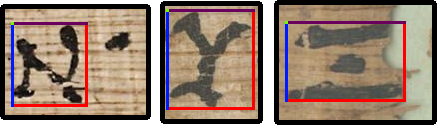
\includegraphics[width=0.75\textwidth]{{bounding/bbox_examples_coco.png}}
    \end{center}
    Three examples of bounding boxes, on a $N$, $\Upsilon$, and a $\Xi$ (left to right). In the COCO bounding box format, bounding boxes are described using the top left corner (marked in green) of the box  in absolute pixels and the box's width (purple) and height (blue) in absolute pixels. In this example, the boxes shown above would be denoted in the COCO format as follows: $N:(6, 13, 76, 84)$, $\Upsilon:(1, 3, 88, 100)$, $\Xi:(6, 16, 120, 80)$.
\end{figure}

\begin{figure}
    \caption{YOLO Format Bounding Box Examples}
    \label{fig:yolobbox}
    \begin{center}
    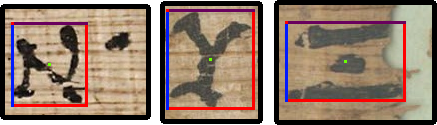
\includegraphics[width=0.75\textwidth]{{bounding/bbox_examples_yolo.png}}
    \end{center}
    Three examples of bounding boxes, on a $N$, $\Upsilon$, and a $\Xi$ (left to right). In the YOLO bounding box format, bounding boxes are described using the center of the box (marked in green) in relative coordinates (based on image width and height) and the box's width (purple) and height (blue) also in relative coordinates. In this example, the boxes shown above would be denoted in the YOLO format as follows (rounded to three decimal places): $N:(0.319, 0.519, , 0.532, 0.739)$, $\Upsilon:(0.469, 0.469, 0.917, 0.885)$, $\Xi:(0.431, 0.487, 0.784, 0.696)$.
\end{figure}

\begin{figure}
    \caption{2D Intersection Over Union (IOU) Examples}
    \label{fig:IOU}
    \begin{center}
      \begin{subfigure}[b]{0.45\textwidth}
           \centering
           \caption{Bounding Boxes With A Low IOU Value}
           \label{fig:lowIOU}
           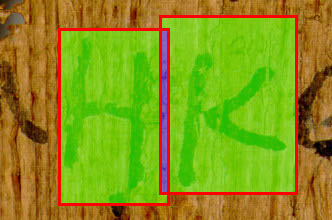
\includegraphics[width=\textwidth]{{bounding/lowIOU.jpg}}
       \end{subfigure}
       \hfill
       \begin{subfigure}[b]{0.45\textwidth}
           \centering
           \caption{Bounding Boxes With A High IOU Value}
           \label{fig:highIOU}
           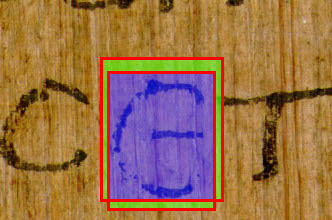
\includegraphics[width=\textwidth]{{bounding/highIOU.jpg}}
       \end{subfigure}
    \end{center}
    The IOU of two bounding boxes is a measure of how similar they are (with a range denoted by the interval $[0,1]$). It is calculated using the following formula, where $a$ and $b$ are bounding boxes represented by sets of pixels.
    \begin{equation}
      \ref{eq:IOU}
      IOU(a,b) = \frac{a \cap b}{a \cup b}
    \end{equation}
    Figure \ref{fig:lowIOU} is an example of two bounding boxes with a low IOU value as the union of the sets (green and blue regions) is much larger than the intersection of the sets (blue region). Figure \ref{fig:highIOU} is an example of two bounding boxes with a high IOU value as the union of the sets (green and blue regions) is similar to the intersection of the sets (blue region).
\end{figure}

\begin{figure}
    \caption{1D Intersection Over Union (IOU) Examples}
    \label{fig:1dIOU}
    \begin{center}
        \begin{subfigure}[b]{0.45\textwidth}
            \centering
            \caption{1D Horizontal IOU Calculation}
            \label{fig:horizonalIOU}
            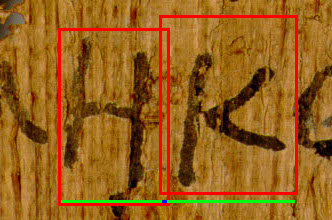
\includegraphics[width=\textwidth]{{bounding/horizontalIOU.jpg}}
        \end{subfigure}
        \hfill
        \begin{subfigure}[b]{0.45\textwidth}
            \centering
            \caption{1D Vertical IOU Calculation}
            \label{fig:verticalIOU}
            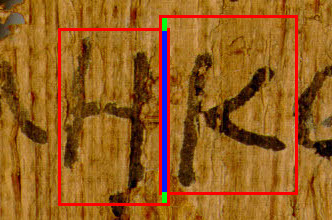
\includegraphics[width=\textwidth]{{bounding/verticalIOU.jpg}}
        \end{subfigure}
    \end{center}
    To find the 1D IOUs of a pair of bounding boxes the boxes each treated as one dimensional objects and the IOU is found as normal, calculating the intersection and union for the $x$ and $y$ dimensions separately. In Figure \ref{fig:horizonalIOU} the horizonal IOU is low, with the intersection of the sets in 1D (blue region) being divided by the union of the sets (green and blue regions). Figure \ref{fig:verticalIOU} has a high vertical IOU, with the intersection of the sets (blue region) being divided by the union of the sets (green and blue regions).
\end{figure}

\subsection{Connected Component Labeling}

Bounding boxes can be generated by the pipeline utilizing a method called connected-component labeling. In this method, which is implemented by OpenCV \cite{OpenCV}, touching similarly colored pixels are grouped together to form blobs in a recursive manner until no more blobs can be grouped. Each blob is given a label and a minimal bounding box (in PASCAL VOC format) that contains the entire blob \seefig{boundingCC}. These bounding boxes are then converted to a bounding box object, which allow them to be utilized by the rest of the pipeline.

\subsection{Region Based Convolution Neural Networks}

Another method for bounding in the pipeline utilizes a region-based convolution neural networks (RCNN) called YOLOv5 \cite{YOLOv5}. The RCNN was trained on the ground truth glyph images in two ways. In the first, YOLOv5 was trained on all twenty-four glyph classes, to allow YOLO to both classify and bound the glyphs. For the second training attempt, the RCNN was trained on glyphs as a single class, preventing YOLO from learning about the separate classes, but allowing it to much more efficiently learn how to bound glyphs and separate them from the noisy background that is papyrus.

Training was preformed utilizing the native YOLOv5 code, downloaded from \href{https://github.com/ultralytics/yolov5}{GitHub}, using the largest network architecture provided (called YOLOv5x). The trained network consists of $~86.7$ million parameters and was trained on mosaic images of glyphs resized to 640px squares over the course of over 600 epochs. After training, the epoch with the best results was extracted and exported for use by PyTorch, which allows the network to be loaded and utilized in the pipeline with no external code required (\textit{see below note for details}).

\textit{Note: YOLOv5 is the product of work by Glenn Jocher (Ultralytics) and hundreds of contributors. I take no credit for the implementation of this network, as all credit for this work should go to Jocher et al. into this project. However, all training and hyperparameter tuning was done by me, as well as integrating the network into this project. The code for YOLOv5 is included in the submission of the project solely to allow the pipeline to function offline, as the network architecture would need to be downloaded from their git repo each time the pipeline was run.}

\subsubsection{RCCN Sliding Window}
\todo{NEW}

Utilizing the YOLOv5x trained network, glyphs can be detected utilizing a sliding window to keep the image sizes closer to the size that the network was trained on. Using an overlapping sliding window with an internal window \seefig{slidingWindow}, full images are split up into smaller images that allow YOLO to bound glyphs and. The bounded glyphs are then accepted if they are in the internal window and added to the list of all glyphs bounding boxes as bounding box objects. Clear outliers and invalid glyph bounding boxes are then be removed by heuristic approaches that clean the list of bounding boxes to generate a list of high-quality potential glyph bounding boxes.

\begin{figure}
    \caption{Sliding Window Region Examples}
    \label{fig:slidingWindow}
    \begin{center}
      \begin{subfigure}[b]{0.3\textwidth}
           \centering
           \caption{Corner Sliding Window Region}
           \label{fig:slidingWindowCorner}
           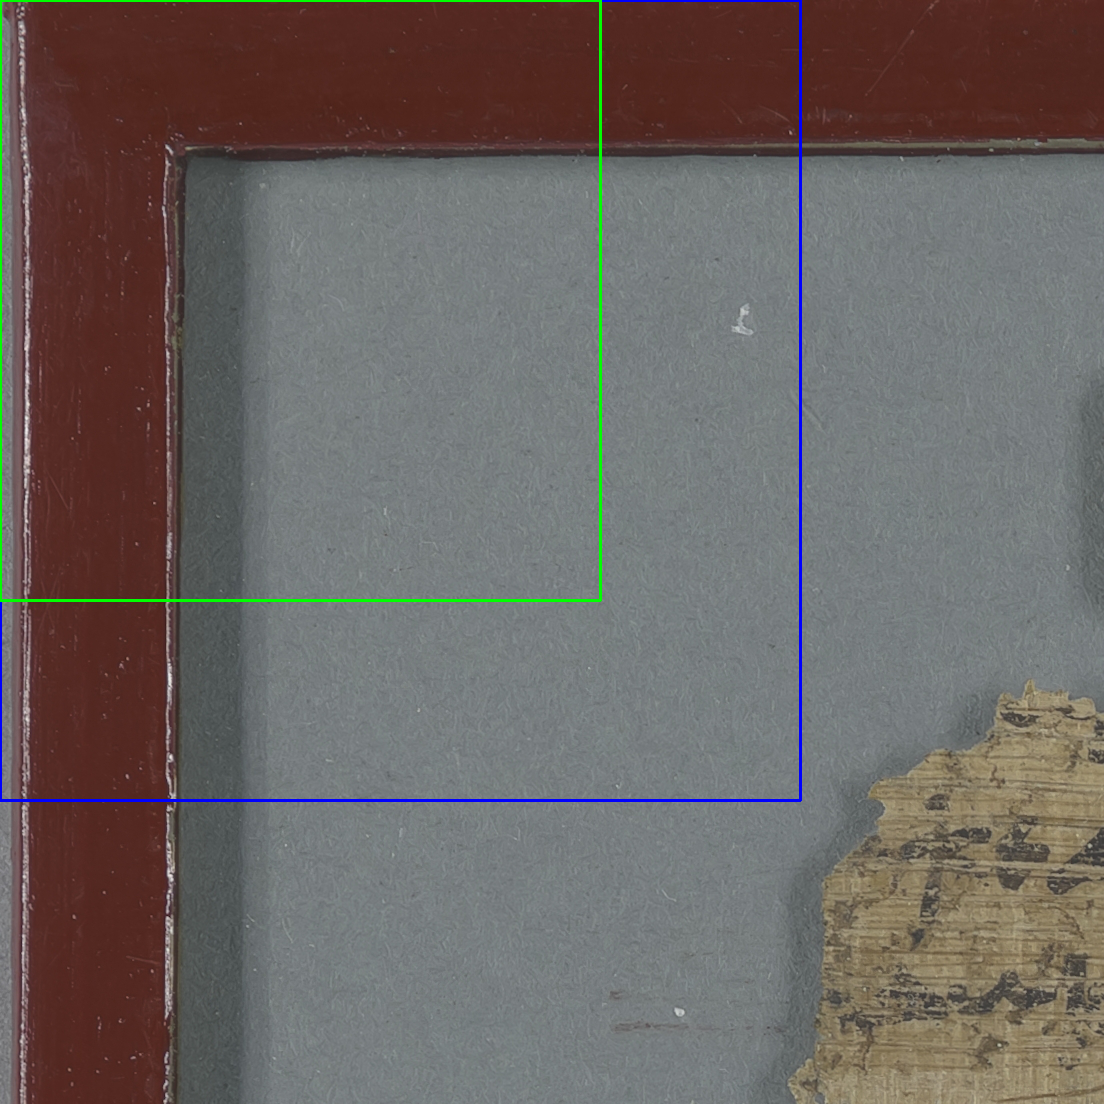
\includegraphics[width=\textwidth]{{bounding/window_0_0.png}}
       \end{subfigure}
       \hfill
       \begin{subfigure}[b]{0.3\textwidth}
           \centering
           \caption{Edge Sliding Window Region}
           \label{fig:slidingWindowEdge}
           \includegraphics[width=\textwidth]{{bounding/window_0_200.png}}
       \end{subfigure}
       \hfill
       \begin{subfigure}[b]{0.3\textwidth}
           \centering
           \caption{Center Sliding Window Region}
           \label{fig:slidingWindowCenter}
           \includegraphics[width=\textwidth]{{bounding/window_600_1800.png}}
       \end{subfigure}
    \end{center}
    Examples of the three cases of sliding window regions. In each image, the blue bordered region represents the region of the image that is given to the CNN to find glyphs in with the green region represents the region of the image that a bounding box must be fully within to be accepted as a valid bounding box. Bounding boxes that are found, but not accepted as valid are marked in red, with valid bounding boxes being marked in black. Bounding boxes marked in black outside of green bounded region are boxes that have already been accepted by other windows in the sliding window collection. In the left-most figure (\ref{fig:slidingWindowCorner}), the region of acceptance is expanded to fit to the corner, as there would otherwise need to be an image that is smaller than the rest to pass into the CNN. For the same reason, the middle figure (\ref{fig:slidingWindowEdge}) shows a region of acceptance that is expanded to fit to the edge of the image. The region in the right-most right (\ref{fig:slidingWindowCenter}) is an example of a normal region, with no expansion required to ensure full coverage of the image.
\end{figure}

\subsubsection{RCNN Duplicate Removal}
\todo{TODO: IMPLEMENT AND DISCUSS, ADD FIGURES}

\subsubsection{Binarization-Assisted CNN}

The close cropping approach based on connected component labeling on binarized images can be conjunction with the larger bounding boxes generated from the RCNN based methods. This allows the bounding boxes generated by the RCNN to be used as initial potential regions, which can then be cropped down to closely fit the glyph they contain \seefig{boundingBinaryAssistedCNN}. This approach to creating tight bounding boxes on binarized images is able to approximate minimal bounding boxes for the raw input images, which would otherwise be difficult to generate tight-to-ink bounding boxes for, as the ground-truth training data is not tightly bound.

\section{Line Bounding}

Once bounding boxes for individual glyphs are generated, they can be grouped together to form lines, which allow the language models in the classification step to have the context in which glyphs appear.

\subsection{Point Of Interest Clustering}

The first approach to line bounding is based on the work of Garz et al. \cite{Garz2011, Garz2012}, which utilizes points of interest to group lines together. In this approach, gaussians and the SIFT algorithm are utilized to find points of interest, which are clustered by the DBSCAN algorithm, with an adaption proposed by Daszykowski et al. \cite{Daszykowski}.

\subsubsection{Difference of Gaussians}

The first step in this algorithm requires that features be extracted from the images in a scale-invariant way, such that any image size may be utilized without the need for scaling, which could cause information to be lost. To do this, the Difference of Gaussians (DOG) method is utilized. Using the implementation of this algorithm provided by OpenCV \cite{OpenCV}, a collection of gaussian kernels is generated and used to blur a greyscale image to extract high frequency spatial data. As multiple gaussian blurs are preformed, only signals in the image that are between the frequencies of the gaussian kernels remain after the differences of the all the gaussian blurred images is taken and used to construct a new image. This results in an image that contains only the high frequency data of the original image, regardless of the size of the original image.

\subsubsection{Points of Interest \& SIFT}

Using the scale-invariant feature transform algorithm (SIFT) \cite{Lowe}, on the high-frequency information extracted by DOG, key points are extracted from the image which are transform, scale, and rotation invariant.

% However, SIFT often creates too many key points, so many are discarded based on their location in the image, removing key points on the edges of objects, allowing the remaining key points to be more optimal for matching and recognition.

\subsubsection{Adaptive DBSCAN}

Once points of interest are generated using SIFT, they are clustered by a scale invariant version of Density-Based Spatial Clustering of Applications with Noise (DBSCAN) \cite{Ester} proposed by Daszykowski et al. \cite{Daszykowski}. This method works by first generating $n$ random points in a region with the same size as the image, where $n$ is the number of points of interest that need to be clustered. Then the distance to the $m$th closest point is found for each point, where $m = \frac{n}{25}$. The $95$th percentile is then taken for these distances, which is used as the $\epsilon$ parameter for DBSCAN (the maximum distance for a point to be added to a cluster), with $m$ acting as the minimum number of points required to form a cluster.

The clusters produced by this method can then be considered to be lines, while points outside of clusters are noise or glyphs that are not within lines.

\subsection{Adjacent and Overlaping Glyph Clustering}

Another method for clustering glyphs is to utilize domain knowledge to link glyph bounding boxes horizontally using close and overlapping bounding boxes. Using this method, glyphs are linked into lines by linking glyphs based on proximity in the x and y directions. Horizontally overlapping bounding boxes are linked if they overlap in they each contain the y coordinate at the center of the other bounding box. Boxes are similarly linked if they are relatively close to each other, based on the average width of the two glyph bounding boxes \seefig{linesOverlap}.

Once rough grouping are generated using this method, the lines are cleaned of extranious and overlarge bounding boxes by removing bounding boxes that have no effect on the validity of the line based on this linking method. Lines are then joined together if possible, to form longer lines.

\subsection{Line Based Bounding Box Cropping}

Once glyphs are linked into lines, the bounding boxes of the glyphs in each line can be cut down such that there is no overlap between bounding boxes. For each pair of overlapping bounding boxes, the center of the overlapping region is set as the edge for both bounding boxes, such that the bounding boxes touch, but do not overlap \seefig{boundingBoxOverlapCrop}.

\section{Train/Test Data Extraction}

\subsection{Ground Truth Glyph Examples}

The ground truth data provided by the contest contained image files, each with multiple bounding boxes and glyphs. To extract this data for the purposes of training and evaluation of classification and bounding methods, each original image was copied and cropped to contain only one glyph, generating a single cropped image, cut to the exact bounding box given, for each glyph \seefig{ground_truth_glyphs}. To extract the isolated glyph images for training, the following method is used. For each image in the training data, the image was loaded, and the COCO file provided by the contest was utilized to find each annotated glyph. For each glyph, the loaded image was duplicated and cropped to the bounding box provided in the COCO file. The cropped image was then saved to file either separated by glyph class, or without any class label.
Each cropped glyph file was saved with information on which image the glyph was cropped from, the style it was written in \seefig{xi_footmarktype}, and the preservation of the glyph \seefig{omega_basetype}.

These methods were used to extract glyph images from both the binarized images and un-altered images. Similar processes were also used to generate training data for the various CNNs, and external tools utilized in the project.

\begin{figure}
    \caption{Ground Truth Glyph Examples}
    \label{fig:ground_truth_glyphs}
    \begin{center}
    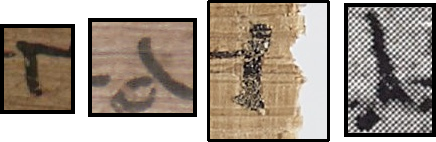
\includegraphics[width=0.75\textwidth]{{glyphs/ground_truth_glyphs.png}}
    \end{center}
    Four examples of the bounded glyphs provided by the contest training data. All the glyphs provided in the training and test data are uppercase and bounded by hand-drawn bounding boxes, which appear here. The first glyph, a $\Gamma$, is well formed, but has the noise from another glyph on the left side and is truncated by the bounding box on the right side. Similarly, the second glyph, an $A$, is well formed, but has the noise from another glyph on the left side and is truncated by the bounding box on the right and bottom sides. The third glyph, an $I$, is not cut off, but does have a line from a neighboring glyph as well. It also shows the edge of the papyrus. The fourth glyph, another $A$, is an example of the varying image quality of the training data, showing obvious artifacting or distortion.
\end{figure}

\begin{figure}
    \caption{Styles of $\Xi$ in the Training Data}
    \label{fig:xi_footmarktype}
    \begin{center}
    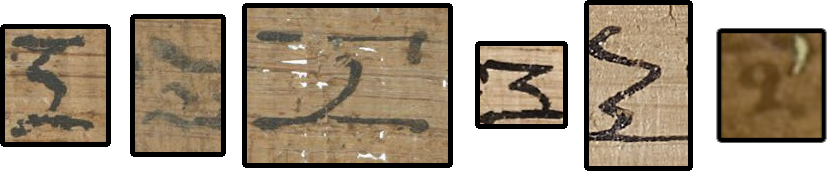
\includegraphics[width=0.75\textwidth]{{glyphs/xi_footmarktype.png}}
    \end{center}
    Examples of the six unique styles for the letter $\Xi$, as determined by the authors of the contest this project was based on. Numbered from 1-6 left to right. The furthest right image of a $\Xi$ was resized for the purpose of display in the figure, which has increased the blurriness of the image.
\end{figure}

\begin{figure}
    \caption{Examples of Preservation Levels in $\Omega$'s in Training Data}
    \label{fig:omega_basetype}
    \begin{center}
    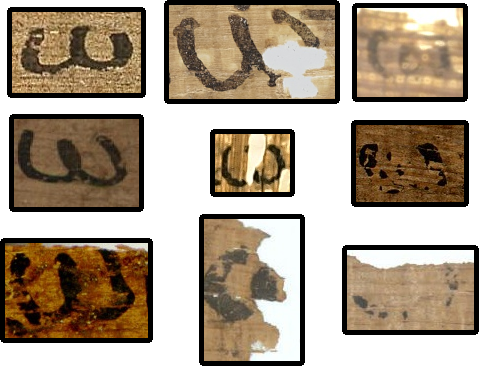
\includegraphics[width=0.75\textwidth]{{glyphs/omega_basetype.png}}
    \end{center}
    Examples of the three levels of preservation for the letter $\Omega$ (appearing as the unical manuscript form, which looks similar to a larger lowercase modern $\omega$), as determined by the authors of the contest this project was based on. Numbered from 1-3, left to right. There are three examples of each level to display three examples of the various degradations that lead to being in each level. The least degraded level (1) is defined as a complete or nearly complete glyph. The second least degraded level (2) is defined as an incomplete letter that unambiguously belongs to one class. The most degraded level in the dataset (3), requires context to determine its actual class, as the glyph may appear to potentially be one of multiple classes when viewed in isolation.
\end{figure}

\subsection{Tightly Bound Glyph Examples}
\todo{NEW}

Using methods described further down, tightly bound glyph images \seefig{fig:cropped_ground_truth_glyphs} were able to be generated and stored for use in training and evaluation using non-arbitrary bounding boxes. After generating bounding boxes, automatically cropped tightly to the glyph, ground truth bounding boxes were paired with the generated bounding boxes and used to automatically assign the known class to the generated bounding box, so the generated bounding boxes could be stored and later utilized for training and evaluation of classification models on real data generated by the pipeline, instead of using the models trained on the ground truth bounding boxes.

\begin{figure}
    \caption{Ground Truth Glyph Examples}
    \label{fig:cropped_ground_truth_glyphs}
    \begin{center}
    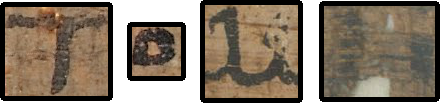
\includegraphics[width=0.75\textwidth]{{glyphs/cropped_ground_truth_glyphs.png}}
    \end{center}
    Four examples of the cropped glyphs generated by the pipeline. The first glyph, a $T$, is well formed and is tightly bounded on all sides besides the top. Similarly, the second glyph, an $O$, is well formed, but has empty space on the bottom and right side. The third glyph, a $M$, is tightly bounded on all sides but the bottom and has degradation. The fourth glyph, an $H$, is poorly formed, with significant amounts of smudging, but is tightly bound on all sides. Glyphs are not reliably tightly bound on all sides, as the center is maintained when cropping, causing up to two sides of a well-formed glyph to have padding. Poorly formed glyphs are sometimes less tightly bound due to issues in their edges.\end{figure}

\subsection{Greek Language Corpus}

To form the training data for a language model, the entirety of the Greek section of the Perseus Digital Library \cite{Perseus} dataset was downloaded. The data was converted from XML to plain text and cleaned of all non-standard Greek letters utilizing a mix of regex, python string functions and a list of the glyphs that appear in the training set of images. When removing invalid characters, the passages that they appeared in were also removed to ensure the integrity of the training data. To ensure the language data was as close to the image training data as possible, all diacritics and punctuation marks were removed, and the letters were converted to their uppercase variant. The remaining data contains $~46,400,000$ glyphs. This data was used to generate five smaller files for the purposes of training language models by randomly selecting chunks from the data.

\section{Classification}

\subsection{Transfer Learning}
\todo{NEW}

Due to the potentially time-consuming nature of developing and training CNNs to classify images, a section of a pre-trained AlexNet \cite{Krizhevsky} was utilized to convert individual glyph images to feature vectors of size $9,216$ to utilize in supervised and unsupervised learning. AlexNet is used as it is a proven network that has shown promise as an engine for image similarity research \cite{Vadicamo, Yuan}. This was done by taking all the convolutional layers of AlexNet and the first fully connected layer and utilizing the output of those layers as a feature vector for the use of various unsupervised learning methods and later neural networks. Images are first shrunk such that their smaller dimension is 240 and then a center crop of size 224 is taken before the pixels are normalized to the distributions expected by AlexNet. All unsupervised methods are based on the implementations by Scikit-Learn \cite{Scikit}. The supervised learning is implemented with PyTorch neural networks \cite{PyTorch}, partially based on the code provided in this PyTorch \href{https://pytorch.org/tutorials/intermediate/torchvision\_tutorial.html}{RCNN training example} and the starter code provided as a part of the contest \cite{Contest}.

\subsubsection{GMM Clustering}
\todo{NEW}

Using the feature vectors generated by AlexNet, GMM clustering on the training data was utilized to generate one gaussian distribution in $N$-dimensional space for each class of glyphs. Using this method, clusters were trained on feature vectors generated from both binarized and un-altered images. The trained clusters can then be utilized to classify unseen feature vectors with the generated chances that a feature vector is the result of an image in each class.

\subsubsection{Random Forest Clustering}
\todo{NEW}

Similarly, using the feature vectors generated by AlexNet, Random Forest Clustering was utilized to generate decision trees in $N$-dimensional space. Using this method, binary decision trees of varied sizes were trained on feature vectors generated from both binarized and un-altered images. The trained trees were then combined and utilized to classify unseen feature vectors with the generated chances that a feature vector is the result of an image in each class with the percentage of decision trees in the forest that pick a class being the likelihood of a feature vector being in that class.

\subsubsection{$K$ Nearest Neighbors}
\todo{NEW}

Finally, a K-Nearest Neighbors network was also generated on the training data. Using this method, feature vectors are classified based on how close they are to feature vectors of known classes. Feature vectors were classified for both binarized and un-altered images. The built networks are utilized to classify unseen feature vectors with the generated chances that a feature vector is the result of an image in each class with the percentage of feature vectors of that class in the K-Nearest neighbors of a given feature vector being the likelihood of a feature vector being in that class.

\subsubsection{Neural Networks}
\todo{NEW}

With the feature vectors output by the modified AlexNet network, it is also possible to train deep neural networks to classify glyphs. Using the size of the feature vector as the input size ($9,216$) and the number of glyphs ($24$) as the output, several dense NNs were generated to classify glyphs, each taking a single feature vector as input and outputing a vector that can be put throught the softmax algorithm to generate a percentage likelihood of the feature vector being from an image of each class of glyph.

\subsection{Convolutional Neural Networks}
\todo{NEW}

Once it was clear that neural networks were out-performing unsupervised learning approaches by a significant margin, CNNs were generated and trained to explore the possibility of further increasing the accuracy of the pipeline. These CNNs are all based on the convolutional layers of pre-trained, and high-preforming CNNS, starting with AlexNet \cite{Krizhevsky} and moving to ResNeXt \cite{Xie}. By extracting the convolutional and pooling layers from these neural networks and attaching a densely connected network on the end with the correct number of output classes, these networks can be adapted to the problem of glyph classification quickly and with minimal training required.

\subsection{LSTM-Based Neural Networks}
\todo{NEW}

LSTM layers are layers in a neural network that allow the model to utilize knowledge of previous and sometimes latter elements in a batch for the classification (or regression) for each input to the network. They work saving an internal hidden state that is altered by and utilized in the output of the layer. These layers can be trained to discard their hidden state or alter their hidden state to increase the accuracy of a model that interacts with ordered information such as language data. These layers can be one-directional, or bi-directional. Bi-directional LSTM layers work by duplicating their input, and mirroring it, generating twice the number of outputs, where half of the output of the layer is assuming the batch was passed in backwards.

Similarly, to the CNNs discussed above, bi-directional LSTM layers can be added to NNs by extracting the convolutional layers from the front of the models and inserting an LSTM layer between the convolutional and the final densely connected layer that generates the output of the model. In addition, densely connected layers can be inserted between the LSTM layer and the convolutional and pooling layers to add an initial classification step before the memory layer and the final classification layer. By utilizing bi-directional LSTM layers, the networks can use the context on both sides of the glyph it is classifying to increase accuracy.

\subsubsection{Training Methodology}
\todo{NEW}

To train these neural networks, techniques to augment the limited ground truth data are utilized. In training, each glyph image is passed into the CNN or NN with a random rotation ($\pm 15^\circ$), perspective ($20\%$), color jitter (brightness$<50\%$, contrast$<50\%$, saturation$<50\%$, hue$<30\%$), and blur ($0-20\%$) applied. When training, images are also grouped into batches using the text in the Perseus dataset to randomly pick glyph images from each class in the order they appear in the ancient Greek language dataset. Models are then trained with dropout $0-50\%$ and ReLU layers between the densely connected layers.

\subsection{Stochastic Language Models}
\todo{NEW}

Using Markov chains, more traditional language models are also trained on the Perseus dataset. Based on the occurrence of glyphs in the dataset, Markov chains are generated to be used in predicting the occurrence of glyphs after or before other glyphs. These models can be utilized with or without log probabilities to generate the likelihood of a string of any given size.

\subsubsection{Partially Observable Markov Decision Process}
\todo{NEW}

Using partially observable Markov decision processes \cite{Astrom} was explored using the pomdp-py python library \cite{Zheng} and the class probabilities given by a language-indifferent classification model. This method allows for Markov states to be defined with uncertainty, allowing for decisions to be made assuming incomplete information. However, there was not time to explore this method further and refine the existing methods, so this method could not be fully explored as a part of the pipeline.
